\chapter{AeroShield}

Téma tejto bakalárskej práce vznikla ako pokračovanie, na už započatom projekte aero kyvadla. Prvá verzia dosky a samotného kyvadla vznikla ako záverečný projekt na predmet Mikroprocesorová technika. Na projekte pracovala pätica študentov: . Schému zapojenia hlavnej dosky, ako aj fotografiu napájkovanej verzie môžeme vidieť na obr.\ref{OBRAZOK 2.1.1}.


\begin{figure}[!tbh]
\centering
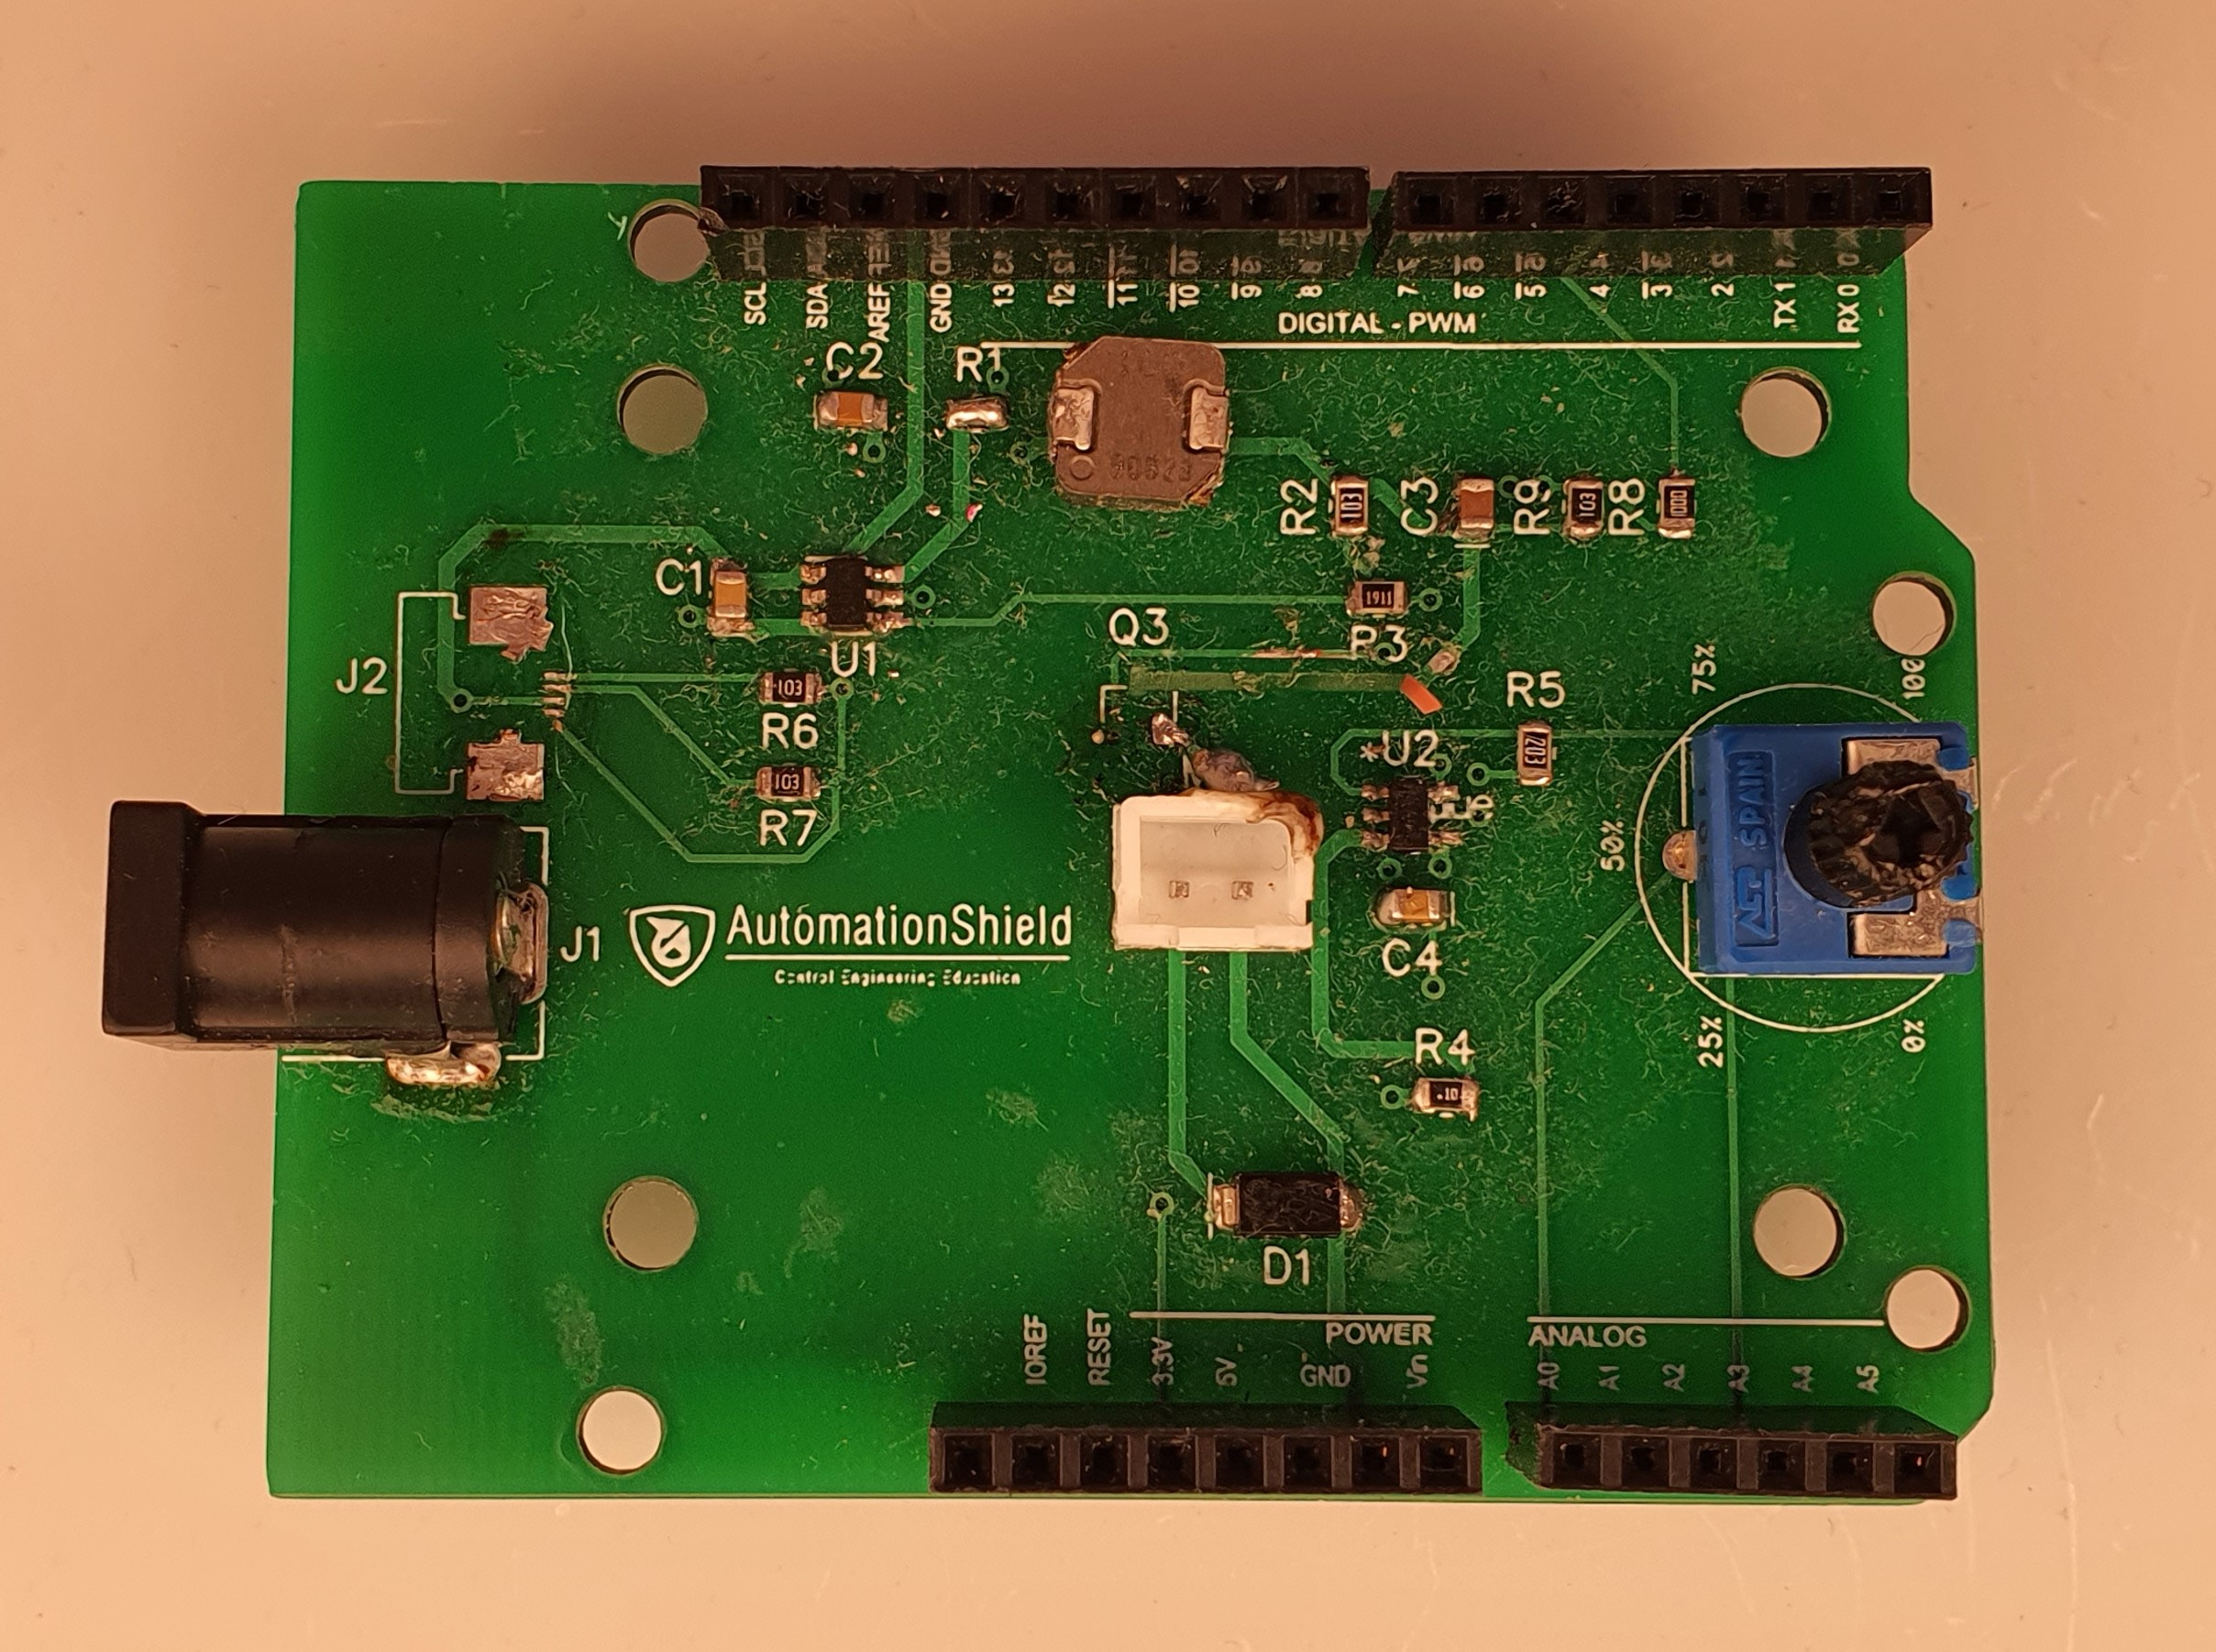
\includegraphics[width=80mm]{obr/oldshield.jpg} 

(a)
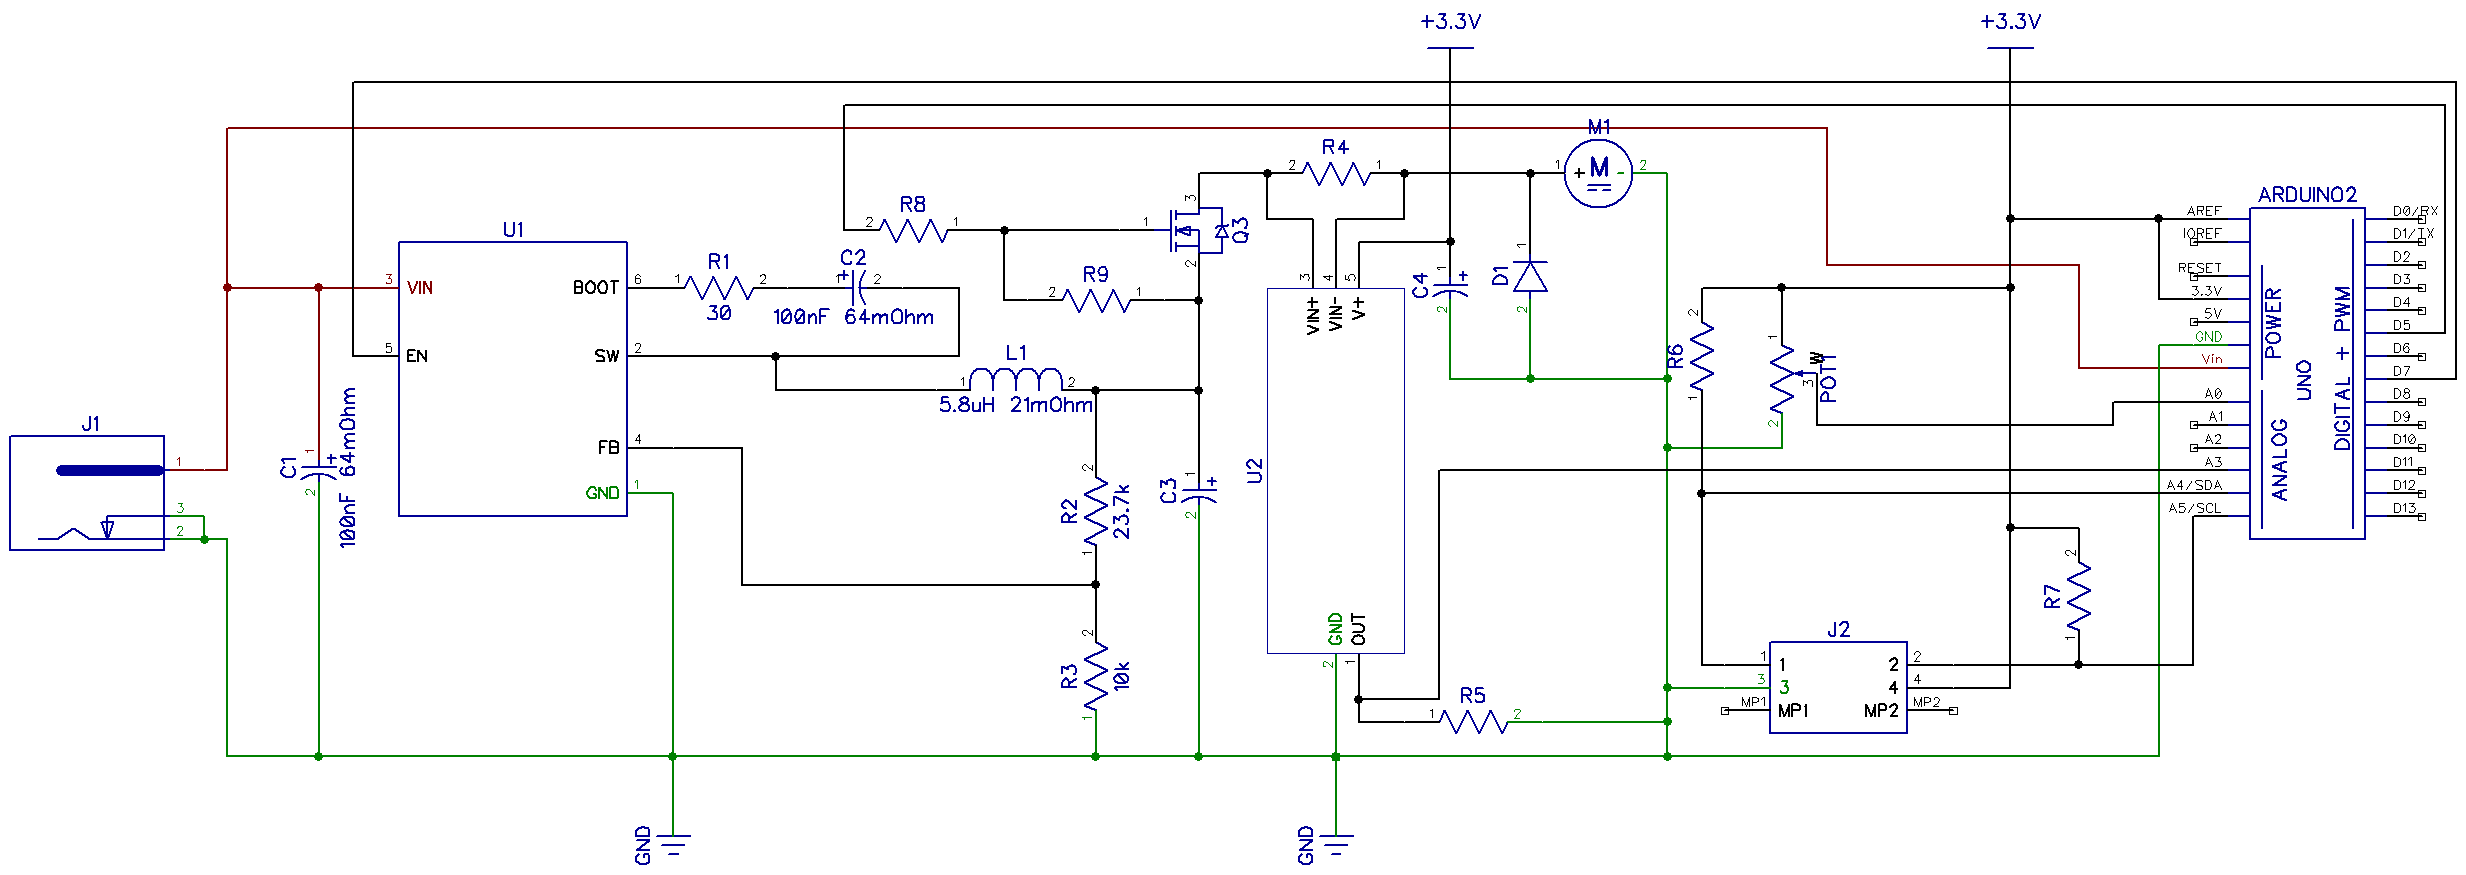
\includegraphics[width=\linewidth]{obr/oldshieldscheme.png}
(b)
\caption{(a) Prvá verzia AeroShieldu. (b) Schéma zapojenia prvej verzie AeroShieldu.}
\label{OBRAZOK 2.1.1}
\end{figure}

\vspace{3cm}

Prvá verzia dosky mala niekoľko nedostatkov, vďaka ktorým bola prakticky nepoužiteľná. Hlavnými nedostatkami boli:

\begin{itemize}
\item neprepojenie pinov komunikácie I2C tj. piny SDA a SCL senzoru hall efektu, ktorý slúži na meranie uhlu natočenia kyvadla,   
\item nesprávne zapojenie mosfetu PMW45EN, ktorý ovláda PWM signál idúci do akčného člena,
\item nesprávne umiestnená ochranná dióda na konektoroch akčného člena, 
\item nesprávne zapojený obvod s čipom INA169, ktorý slúži na meranie prúdu,
\item neprepojenie nulového konektora shieldu s nulovým konektorom arduina.
\end{itemize}

Základom tejto bakalárskej práce teda bolo najskôr pochopiť jednotlivé časti zapojenia, analizovať chyby a ich následná oprava. V rámci školského projektu bola vytvorená hlavná doska na ktorej sa nachádza väčšina elektroniky, avšak bola vytvorená aj verzia menšej dosky ktorá slúži na fungovanie senzoru hall efektu. Táto doska fungovala bezproblémovo a teda netrebalo nijakým spôsobom meniť jej schému zapojenia. Tejto menšej doske sa budeme bližšie venovať v časti\ref{}, no jej podoba je viditelná na obr.\ref{OBRAZOK 2.1.2}.
 
 \begin{figure}[!tbh]
\centering
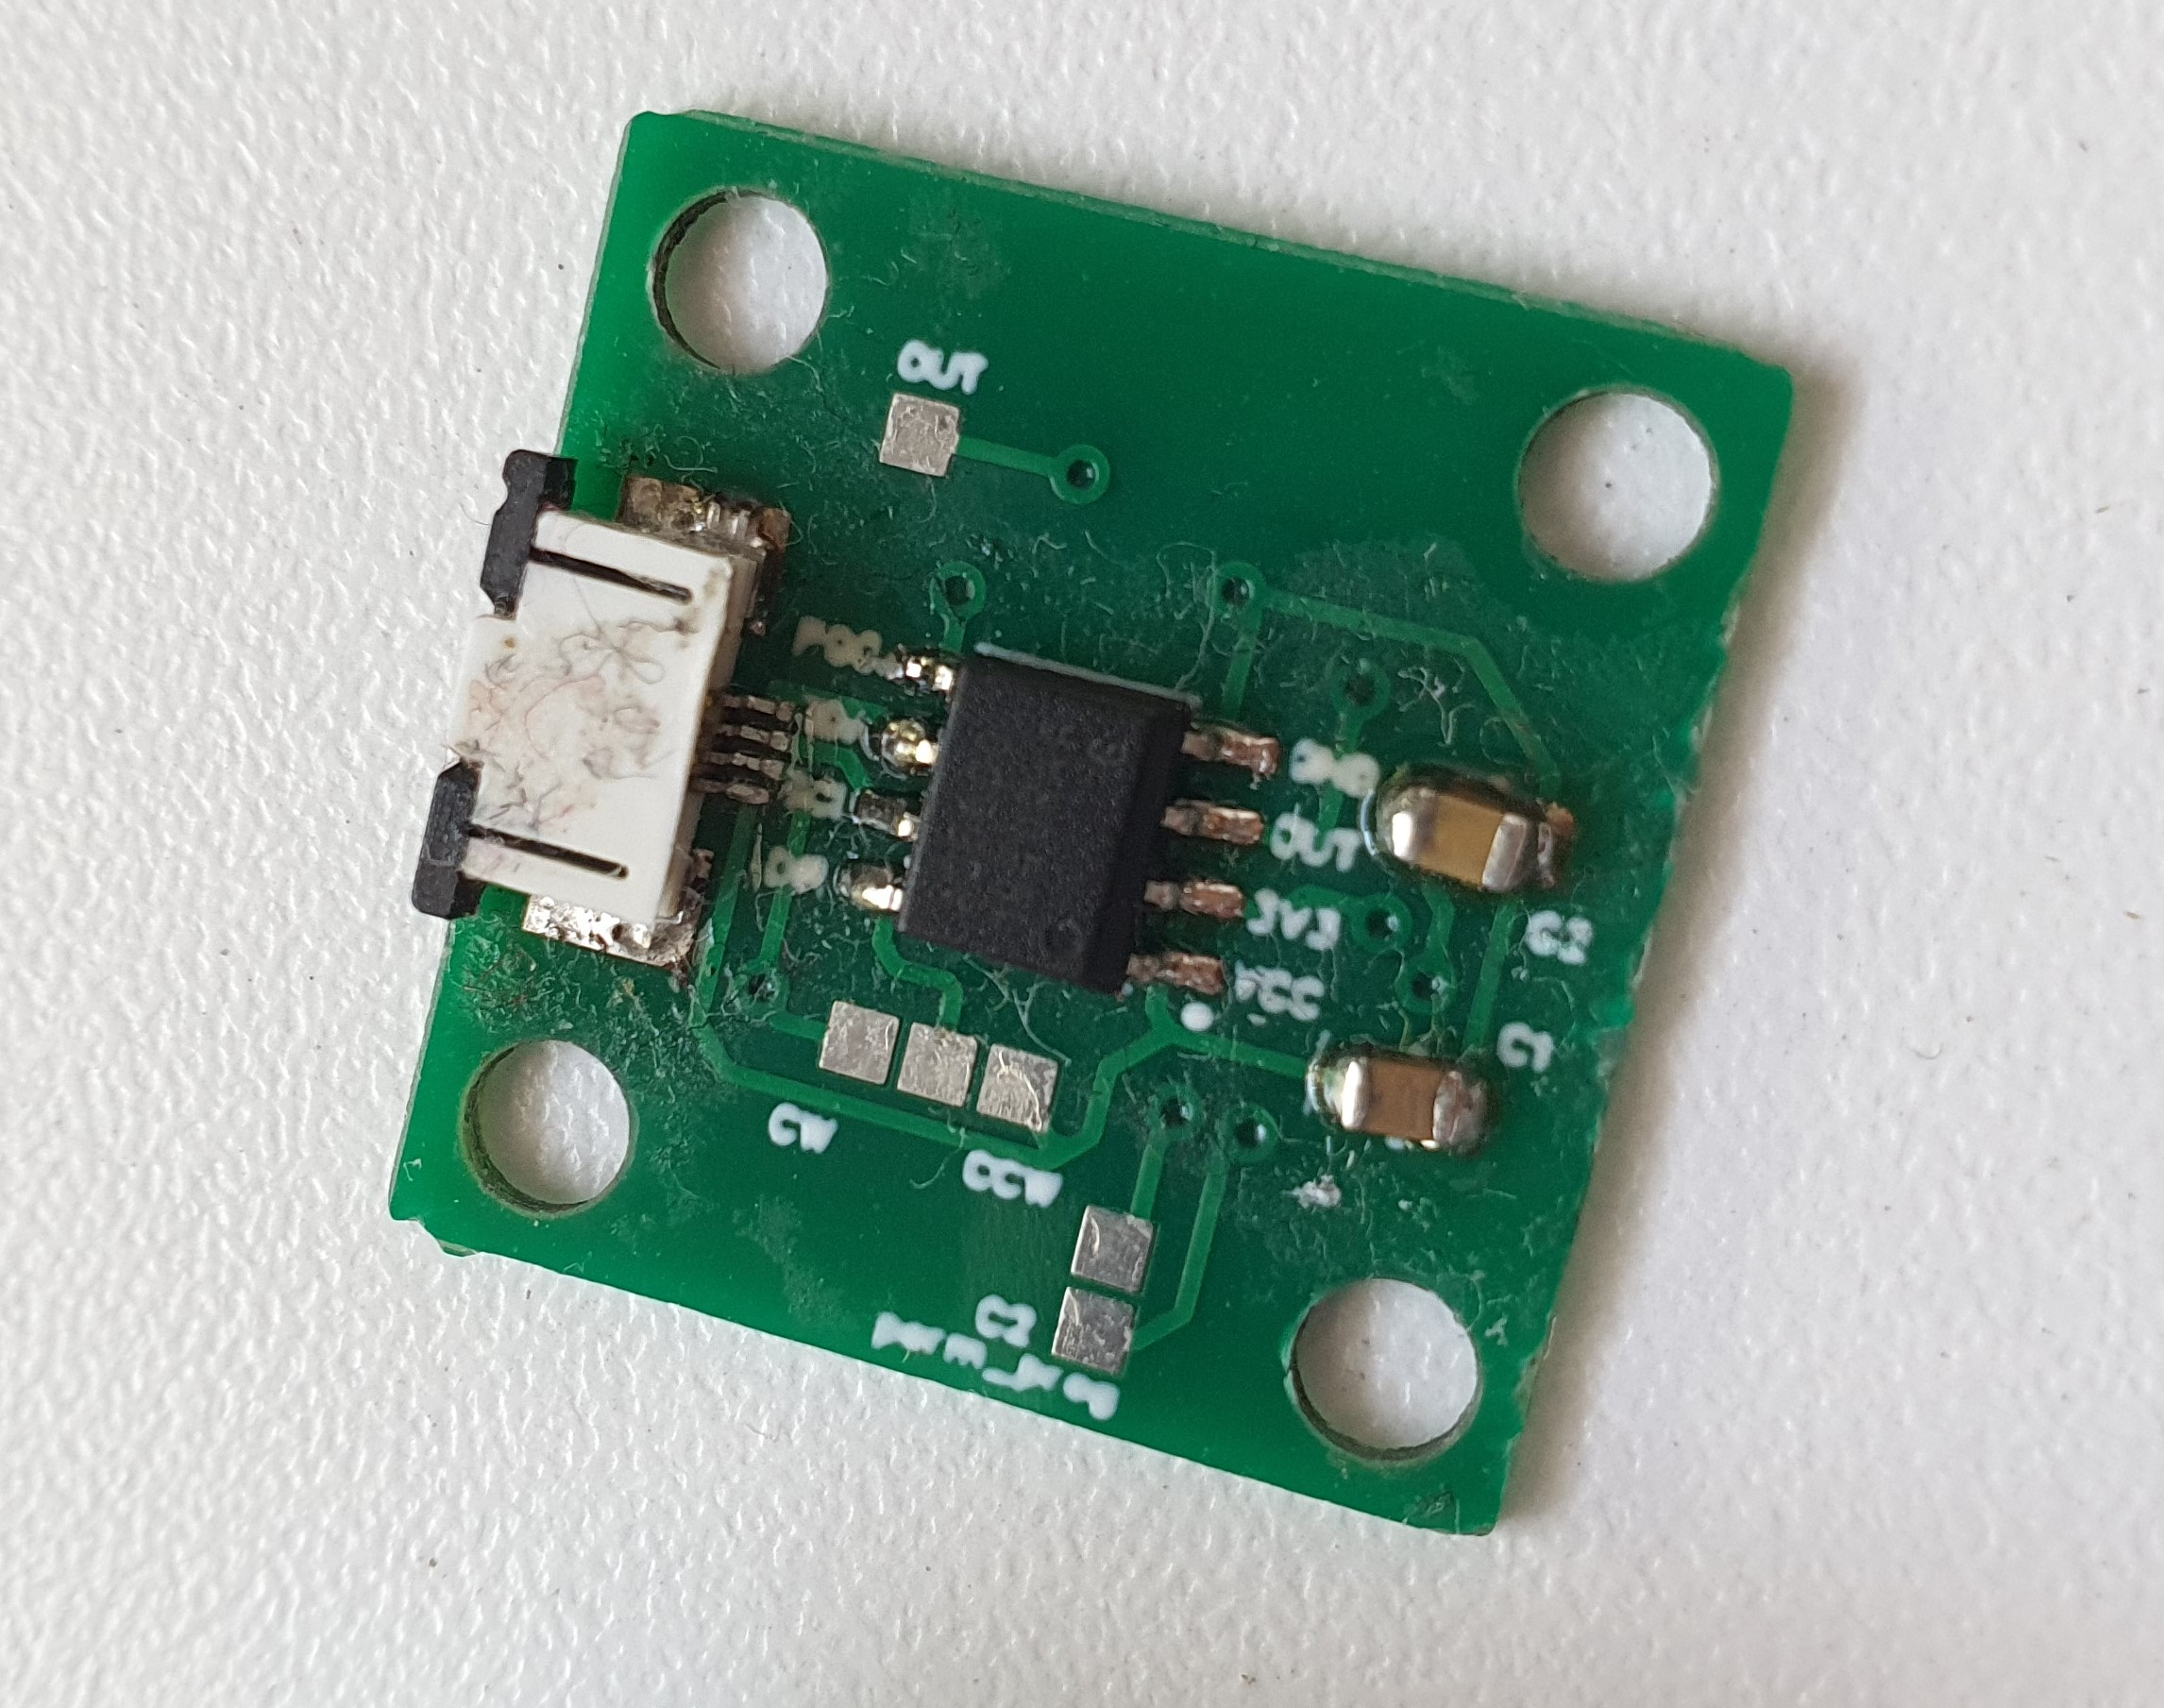
\includegraphics[width=100mm]{obr/breakout.jpg}
\caption{Doska slúžiaca na fungovanie senzoru hall efektu.}\label{OBRAZOK 2.1.2}
\end{figure}

\vspace{3cm}


\section{Hardware}
\subsection{Popis súčiastok}

V tejto časti sa bližsie pozrieme na jednotlivé nevyhnutné súčasti zapojenia AeroShieldu. Konkrétne sa jedná o tieto prvky:
\begin{itemize}
\item napájanie,
\item ovládanie akčného člena,
\item meranie prúdu,
\item meranie uhla natočenia kyvadla,
\item iné.
\end{itemize}


\subsubsection{Znižovanie napätia}
\label{nap}

Na správne napájanie akčného člena, motorčeka, potrebujeme napätie v rozmedzí 0-3,7V. Na shield je však privázdané, pomocou koaxiálneho napájacieho konektora, napätie 12V ktoré by motor v priebehu chvíle zničilo. Potrebujeme preto spôsob ako znížiť privádzané napätie, no súčastne neznížiť privádzaný prúd potrebný na pohon motorčeka. Na tieto účely slúži takzvaný buck converter alebo konvertor na zníženie napätia. Hlavnou Časťou konvertora je čip TPS56339 od výrobcu Texas Instruments obr.\ref{OBRAZOK 2.1}.b. Znižovanie napätia funguje za pomoci dvoch integrovaných N-kanálových 70-m$\Omega$ a 35-m$\Omega$ high-side mosfetov\footnote[4]{N-kanálový mosfet je typ mosfetu, v ktorom tok prúdu nastáva kvôli pohybujucím sa, záporne nabitým elektrónom. "High-side" znamená, že prúd prechádza z napájania, cez mosfet do záťaže a potom do zeme} a dalších komponentov. Celkový prevádzkový prúd zariadenia je približne 98$\upmu$A, keď funguje bez spínania a bez záťaže. Keď je zariadenie vypnuté, napájací prúd je približne 3$\upmu$A a zariadenie umožňuje nepretržitý výstupný prúd do 3 A\cite{buckobr}.

\begin{figure}[!tbh]
\hfill
\subfigure[Schéma zapojenia konvertora napätia.]{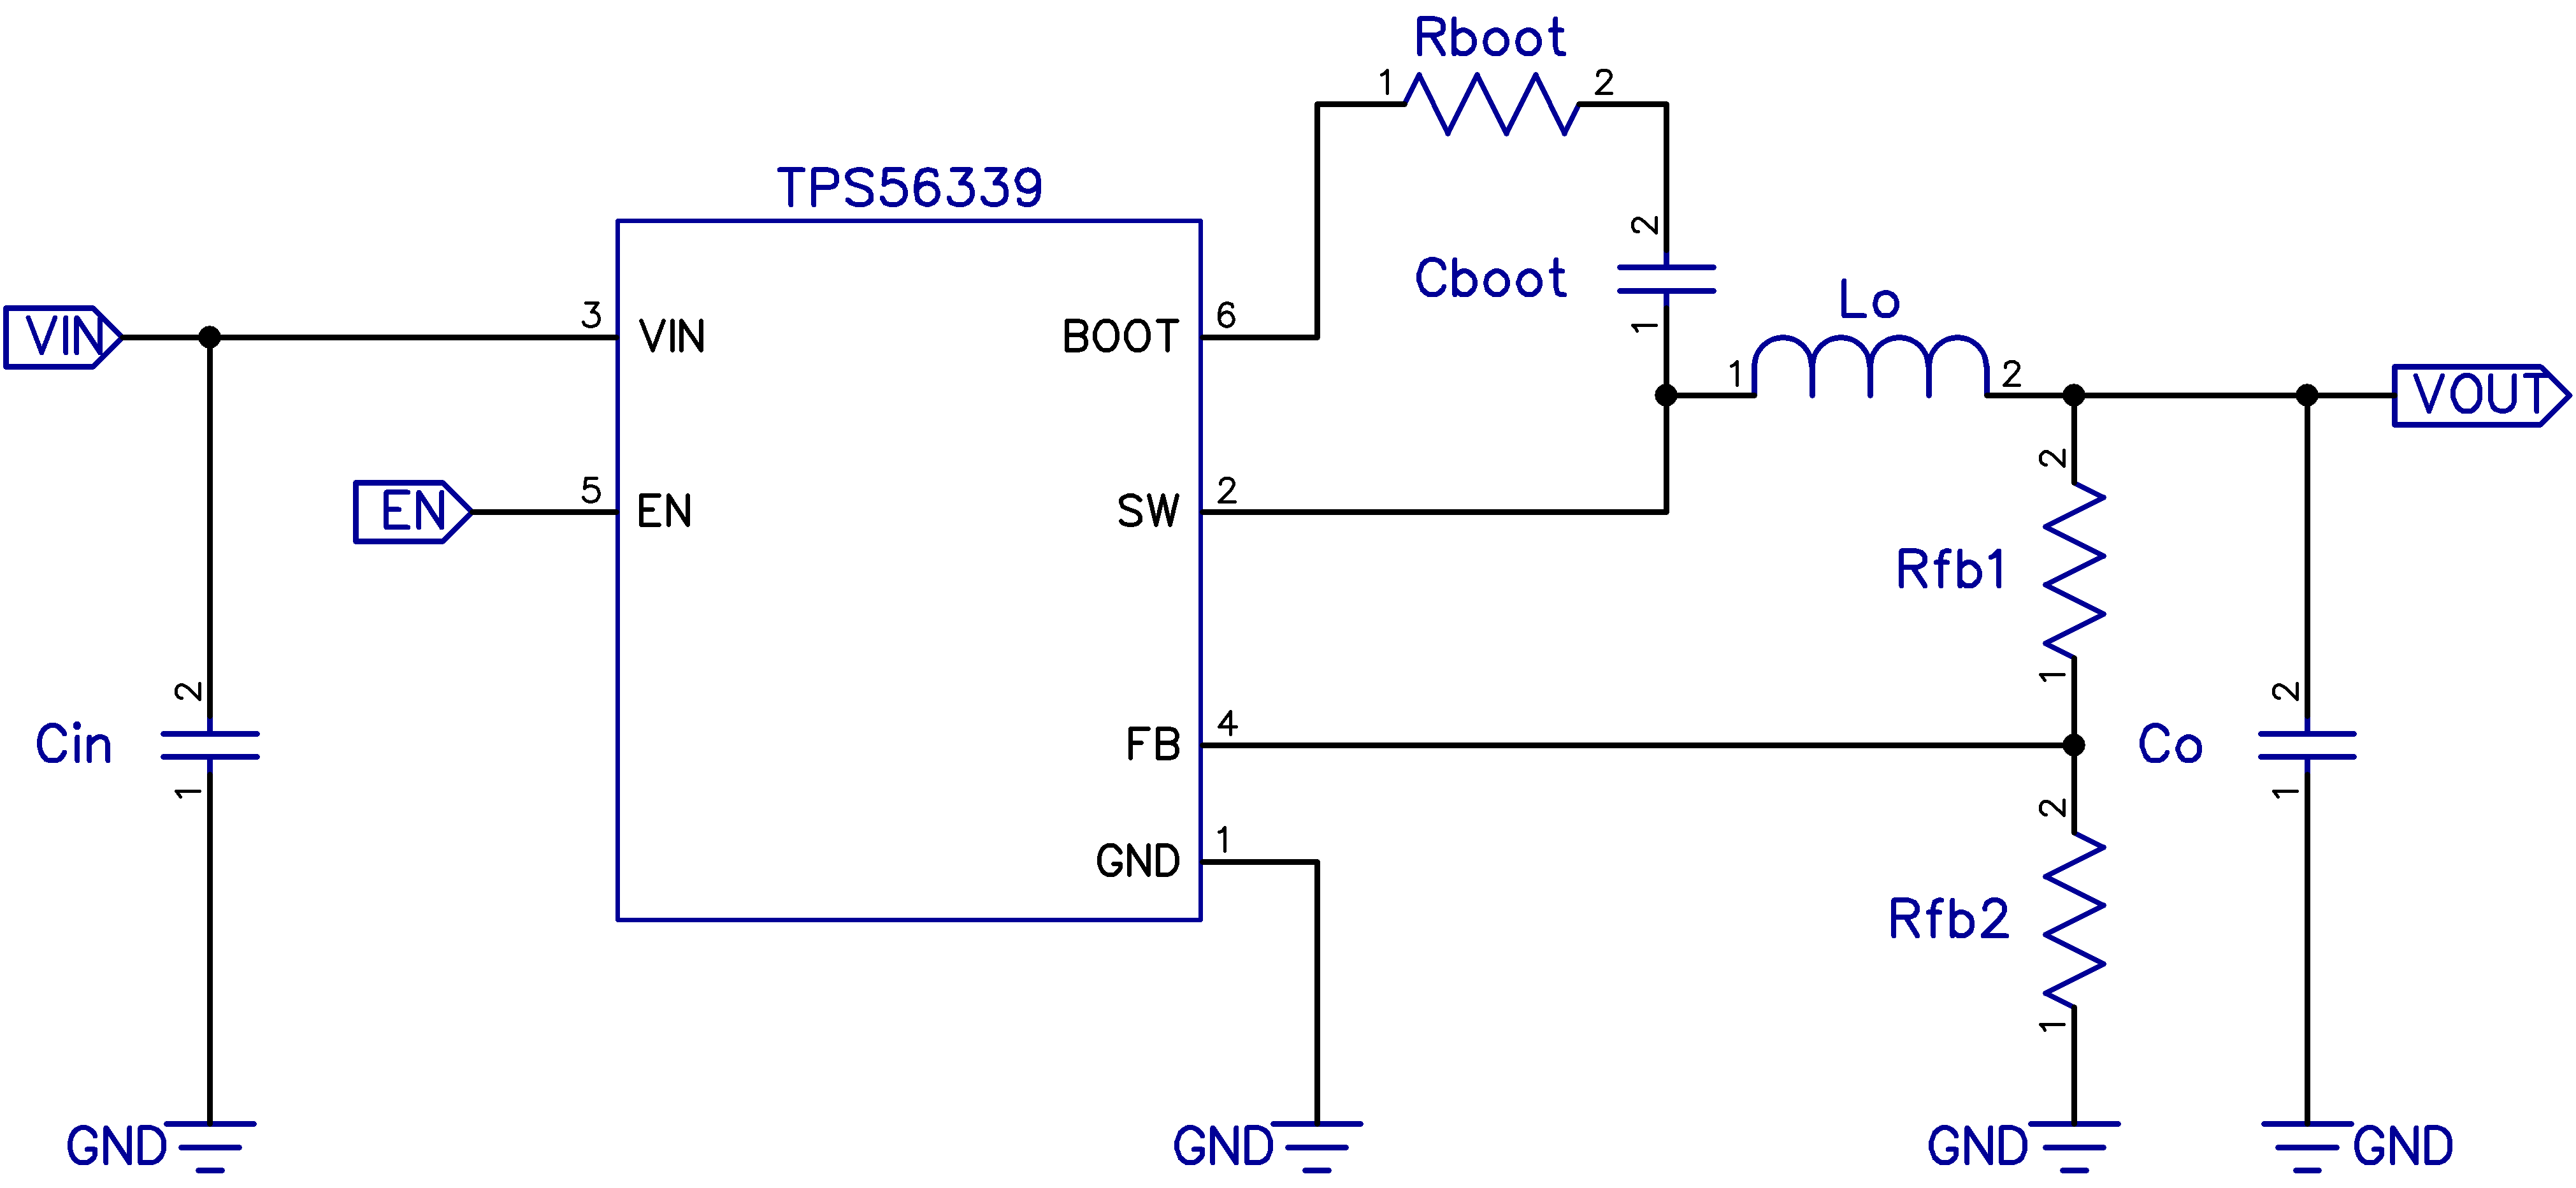
\includegraphics[width=9cm]{obr/schemaBuck.png}}
\hfill
\subfigure[{čip TPS56339\cite{buckobr}}]{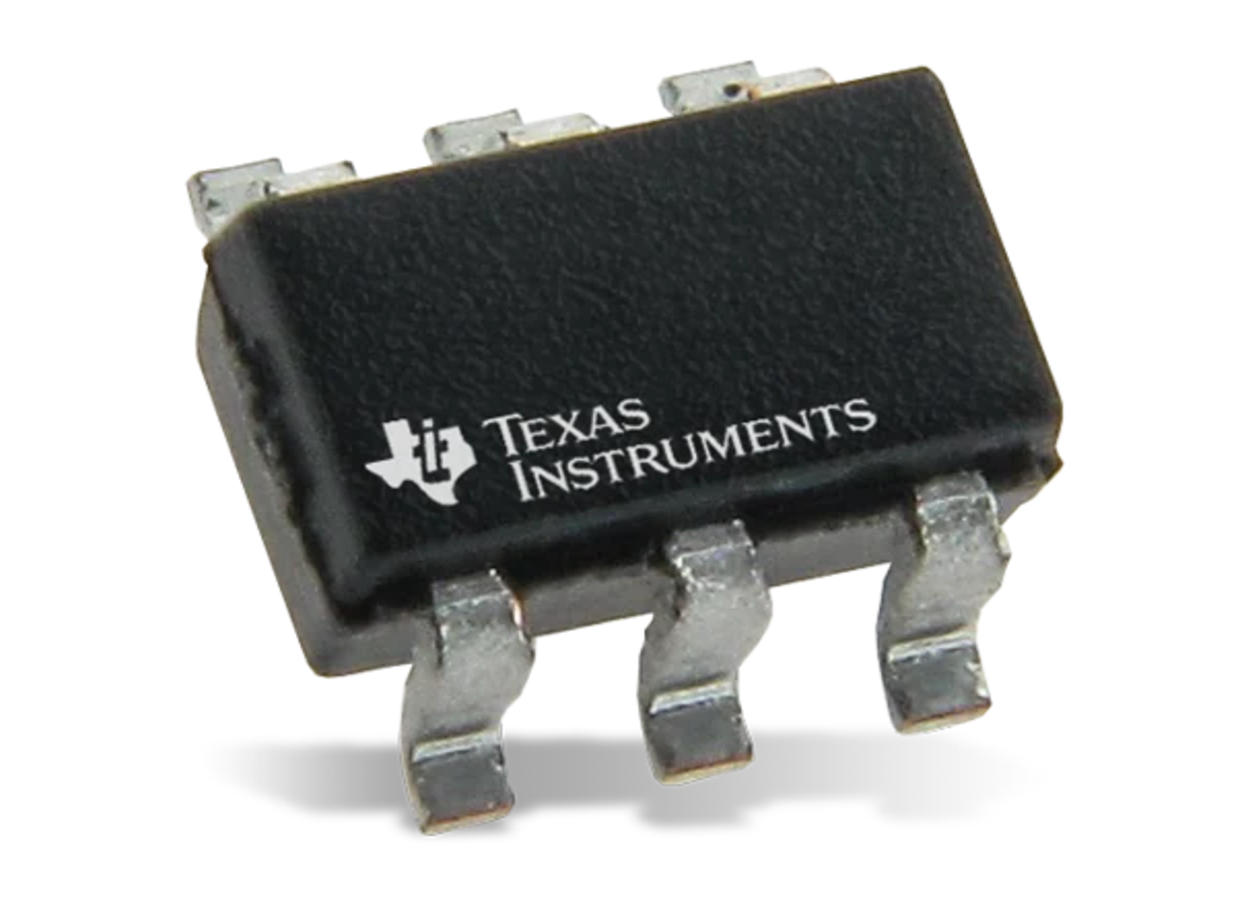
\includegraphics[width=5cm]{obr/cip.eps}}
\hfill
\caption{buck converter}\label{OBRAZOK 2.1}
\end{figure}

 Na čip je privádzané napätie 12V ktoré sa pomocou zapojenia, vididelného na schéme obr.\ref{OBRAZOK 2.1}.a, znižuje na napätie 3,7V. Napájanie motora musí byť realizované externe pomocou koaxiálneho napájacieho konektora, z dôvodu vysokého prúdu odoberaného motorom počas vysokého zaťaženia. Rovnaký konektor sa síce nachádza aj na doske Arduino UNO a pomocou VIN pinu sa dajú napájať napätím 0-12V aj iné zariadenia, avšak tento pin je napojený na diódu obmedzujúcu prúd na 1A\cite{ampere}\cite{ampere2}.



\subsubsection{akčný člen}
\label{akcclen}

akc clen motor hovor bam!
neviem aky mam motor :(
poriesime

PWM 

\vspace{4cm}

\subsubsection{meranie prúdu}
\label{merprud}

Pre čo najpresnejšie ovládanie akčného člena sústavy, motora, je dobré vedieť nie len napätie, ktorým je motor ovládaný, ale aj prúd, ktorý motor odoberá. Na tieto účely sa používajú monitory prúdu, takzvané ("current shunt monitors"). V AeroShielde je použitý snímač INA169NA/250 od výrobcu Texas Instruments obr.\ref{OBRAZOK 2.3}.b.

INA169 je "high-side current monitor", čo znamená, že na kladnú stranu je umiestnený špeciálny rezistor ("shunt resistor") a INA169 meria úbytok napätia na tomto rezistore obr.\ref{OBRAZOK 2.3}.a. Na základe nameraného úbytku napätia vysiela senzor určité napätie ktoré sa následne znásobuje a toto napätie môžeme zaznamenávať. Pomocou základnej matematiky udáva výstupné napätie prúd pretekajúci cez shunt rezistor\cite{INA}.

\begin{figure}[!tbh]
\hfill
\subfigure[Schéma zapojenia snímača prúdu.]{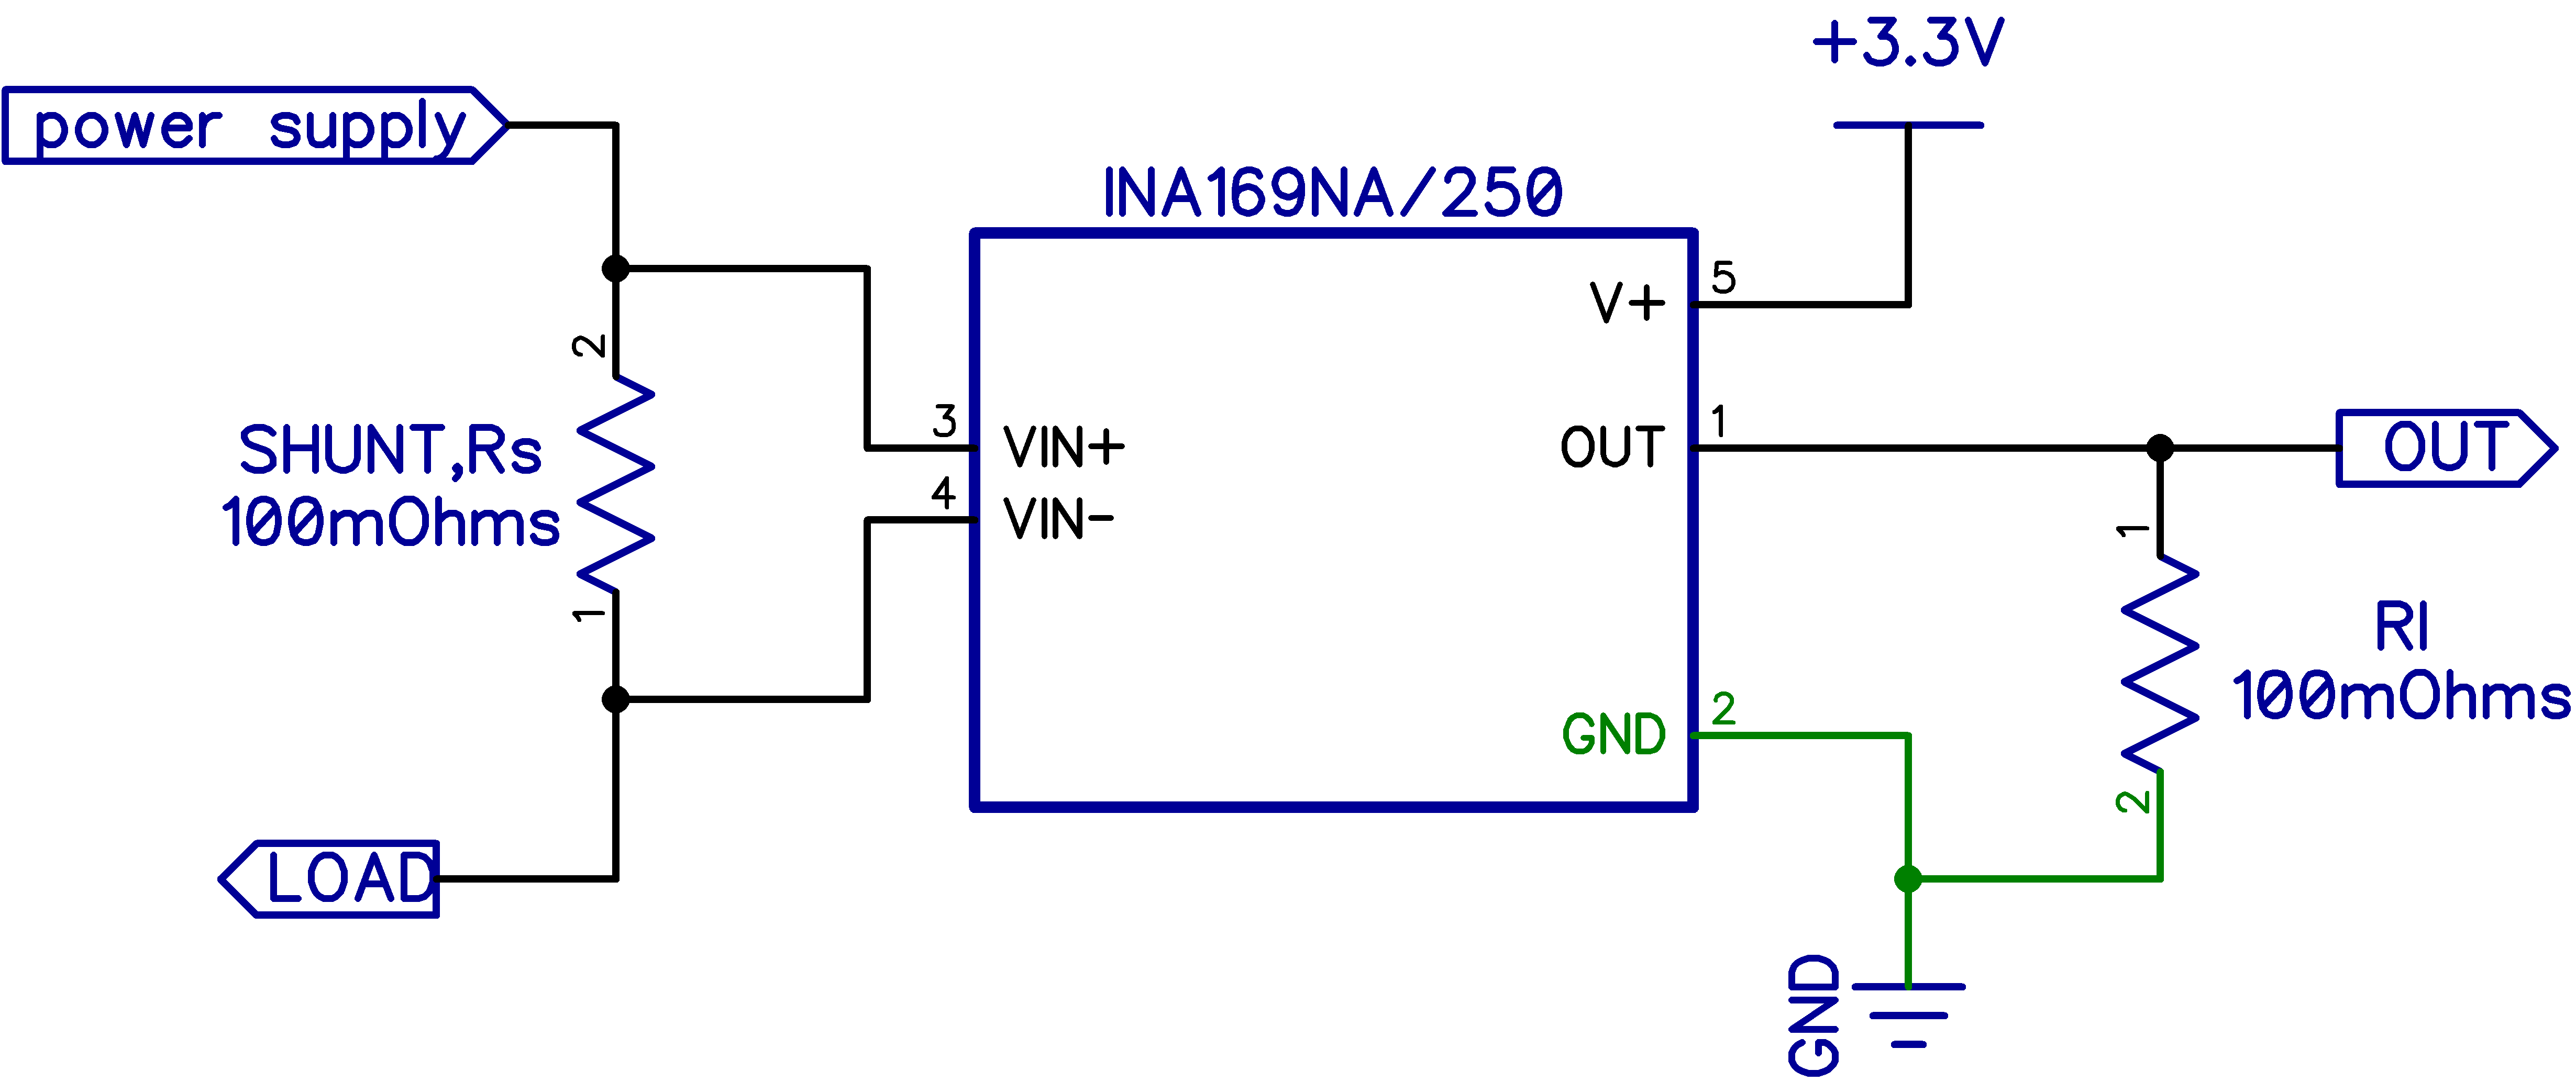
\includegraphics[width=9cm]{obr/INAschema.png}}
\hfill
\subfigure[{Senzor INA169NA/250\cite{INAobr}}]{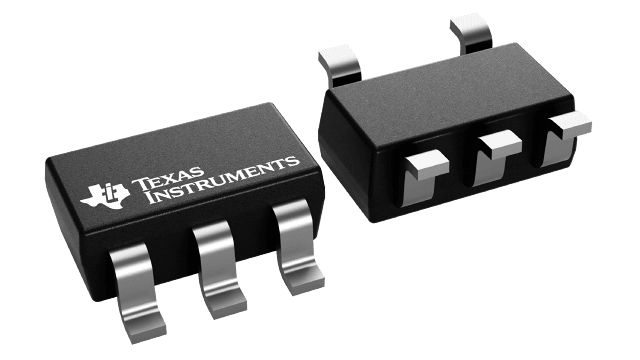
\includegraphics[width=6cm]{obr/ina.png}}
\hfill
\caption{meranie prúdu}\label{OBRAZOK 2.3}
\end{figure}


\label{Hall}
\pagebreak 

\subsubsection{meranie uhla kyvadla}
\label{meruhl}

Na správne fungovanie AeroShieldu je dôležité vedieť s vysokou presnosťou merať uhol naklonenia kyvadla. Na tento účel sme si zvolili meranie uhlu bezkontaktnou formou, pomocou snímača na princípe hallovho javu. Hallov jav vieme opísať ako vznik priečneho elektrického poľa v pevnom materiáli, keď ním preteká elektrický prúd a tento materiál je umiestnený v magnetickom poli, ktoré je kolmé na prúd\cite{Hall}. Toto elektrické pole resp. vznik elektrického potenciálu vieme detegovať a na základe jeho zmeny vieme určit rotáciu kyvadla. V kyvadle je na konci horizontálneho ramena umiestnený špeciálny magnet kruhového tvaru ktorý je polarizovaný naprieč prierezom magnetu.

Ako senzor na meranie hallovho efektu je použitý AS5600 od výrobcu OSRAM obr.\ref{OBRAZOK 2.2}.b. Signály prichádzajúce zo snímača sa najprv zosilnia, následne sú filtrované a prechádzajú konverziou pomocou analógovo-digitálneho prevodníkom (ADC). Výstup ADC je spracovaný pomocou bloku CORDIC (Coordinate Rotation Digital computer) ktorý slúži na výpočet uhla a veľkosti otáčok vektora magnetického poľa. Snímaná je aj intenzita magnetického poľa ktorá sa ďalej používa na
automatické riadenie zosilnenia (AGC) ktoré slúži na kompenzáciu teploty a veľkosti magnetického poľa, ktoré sa mení na základe vzdialenosti magnetu od senzoru.

Na výber sú dva typy výstupu a to analógový výstup alebo digitálny výstup s kódovaním PWM. Senzor má taktiež aj možnosti interného programovania pomocou rozhrania I2C. 
V našom prípade používame 12-bitový analógový výstup s rozlíšením 0°5'16". Toto rozlíšenie nám umožnuje s vysokou presnosťou kontrolovať naklonenie kyvadla a na základe získaných informácii ovplyvňovať fungovanie akčného členu sústavy. Schéma zapojenia čipu na meranie uhlu môžeme vidieť na obr.\ref{OBRAZOK 2.2}.a.


\begin{figure}[!tbh]
\hfill
\subfigure[Schéma zapojenia čipu na meranie uhlu.]{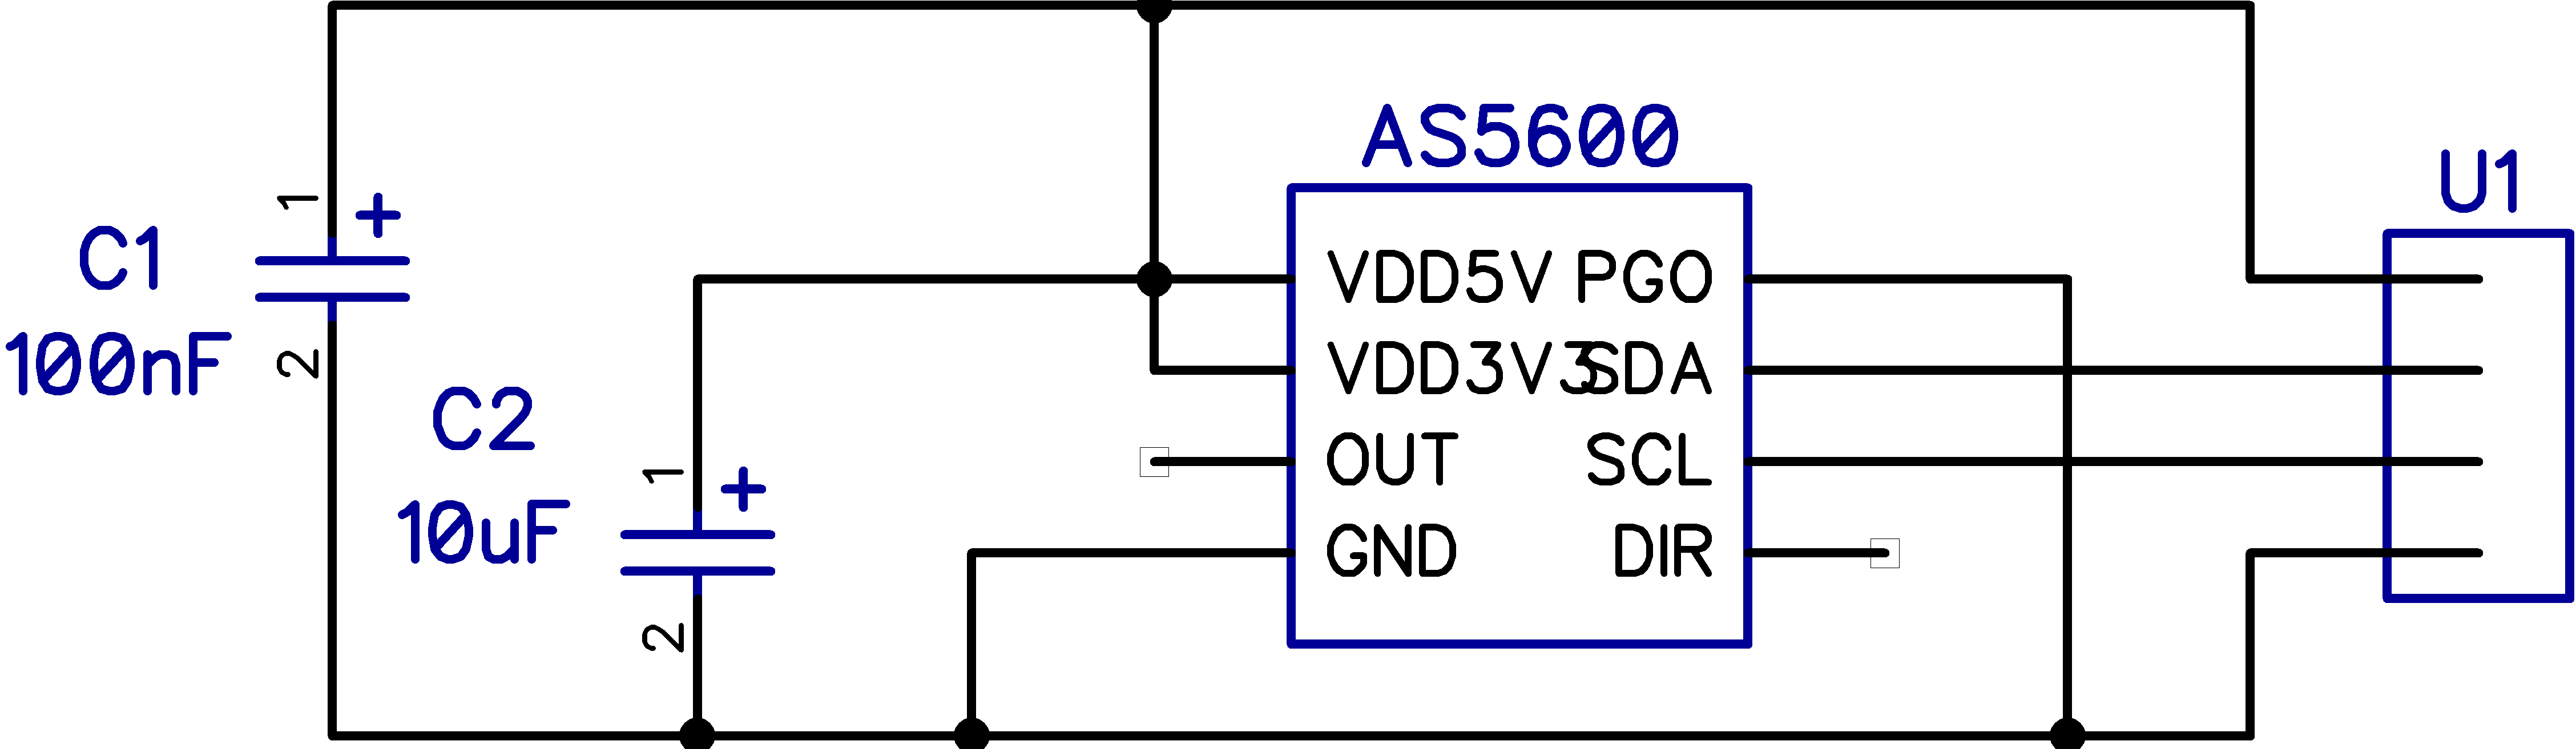
\includegraphics[width=10cm]{obr/as5600.png}}
\hfill
\subfigure[{čip AS5600\cite{As5600obr}}]{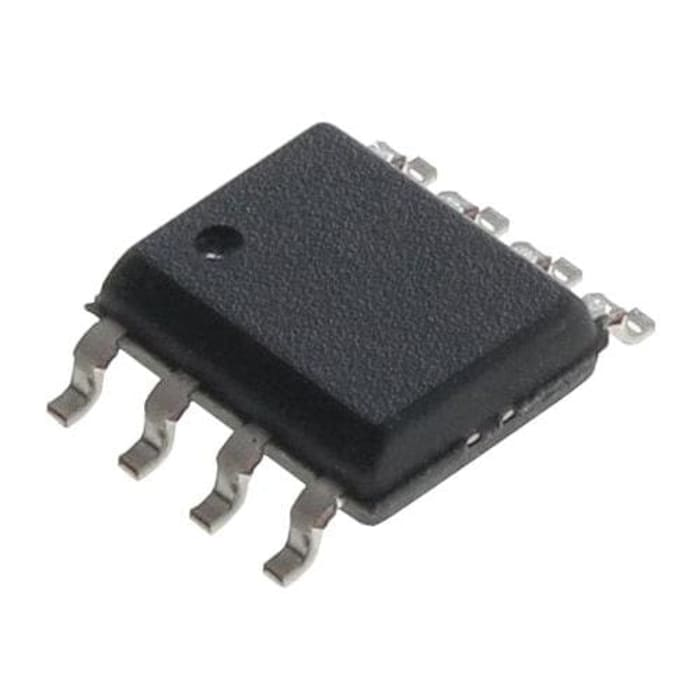
\includegraphics[width=5cm]{obr/hall.jpg}}
\hfill
\caption{meranie uhla kyvadla}\label{OBRAZOK 2.2}
\end{figure}

\subsubsection{ďaľšie dôležité súčasti obvodu}
\label{ine}

potenciometer a mosfet spomeň

\subsection{Schéma zapojenia}

ZAPOJENIE HOVOR O DIPTRACE!

\subsection{Doska plošných spojov}

ZAPOJENIE HOVOR O PLOŠÁKOCH !

AJ BREAKOUT BOARD!

\section{Software}
fgdfgbh 